\setRL
\clearpage
\pagenumbering{arabic} 



در این بخش تمام اطلاعات مدل‌سازی غشای لیپیدی را می‌نویسم.


\section{
بررسی مدل‌ها شبیه‌سازی غشای سلولی.
}
\subsection{
بیولوژی غشا و ساختار آن
}
\subsection{
بررسی مدل گومپر-کرول
}
همانند بخش‌های دیگر فیزیک مانند دینامیک شاره‌ها و نظریه‌ی رسانایی در فلزات، نظریه‌ی پوسته‌های نازک می‌خواهد فیزیک اختلال‌های کُند را بر حسب چند پارامتر ماکروسکوپیک بیان کند. البته که بارها نشان داده شده که چنین نظریه‌هایی به شکل‌ جالبی فروپاشی می‌کنند. مانند با توجه به نظریه جفت شدن مُود‌ها و نظریه باز به هنجارش، افت و خیز‌ها گرمایی باعث می‌شوند که وشکسانی برشی
\LTRfootnote{shear viscosity}
شاره‌های تراکم ناپذیر در ۲ بعد به صورت لوگاریتمی با افزایش اندازه سیستم به بی نهایت میل می‌کند 
\cite{gomppernelson2012}
. غیر خطی شدن رفتار در مورد پوسته‌ها و صفحه‌های نازک نیز اتفاق می‌افتد. افت و خیز گرمایی می‌توانند بر ساختار پوسته‌هایی میکرونی به شدت تاثیر بگذارند زیراکه انرژی خمشی لازم برای بیشتر تغییر شکل‌های پوسته‌های خیلی نازک که زخامت آنها در مقیاس نانومتر است، حدود $k_BT$ است که در اینجا $k_B$ ثابت بولتزمن و
$T$
دماست. مکانیک آماری غشاها و صفحات تخت در گذشته بسیار دقبق مورد مطالعه قرار گرفته. در این سیستم‌ها نشان داده شده‌است که افت و خیز گرمایی در غشاهای تخت باعث می‌شود که مدول کشسانی درون صفحه‌ای
\LTRfootnote{in-plane}
 تابع اندازه‌‌ی سیستم باشد و در اندازه‌های بزرگ به سمت صفر میل کند در حالی که مدول خمشی به بی‌نهایت میل می‌کند. این پدیده‌های ناهنجار ناشی از جفت شدگی غیر خطی میان تغییر شکل‌های خارج از صفحه‌ای (عمود بر صفحه) و تنش‌هایی داخل صفحه‌ی که ایجاد می‌کنند که هنگام تغییر شکل خارج از صفحه از مرتبه‌ی دوم هستند. حتی اطلاعات کمتری در مورد تاثیر افت و خیز گرمایی بر غشا‌های کروی موجود است (شکل 
 \ref{fig:mem1}
)
ولی جفت شدگی بین تغییر شکل‌های روی سطح و عمود بر سطح با یکدیگر تفاوت دارند. به علت وجود هندسه‌ی بسته‌ی غشاهای شبه کروی تغییر شکل حتما همراه با ایجاد کشش در سطح است. در نتیجه جابجایی عمود بر سطح به شکل جملات مرتبه‌ی اول در تنش موازی با صفحه ظاهر می‌شوند. در نتیجه جفت‌ شدگی‌های غیر خطی متفاوت با غشای تخت ایجاد می‌‌شود.

انرژی کشسانی تغییر شکل غشا به شعاع
 $R$ 
با نظریه‌ی پوسته‌های نازک کم عمق مدل‌سازی می‌شود. با این روی‌کرد صحبت از فرورفتیگی‌ها یا برآمدگی‌هایی است که نسبت به بخش مورد مطالعه کوچک هستند. جابجایی درون صفحه با فنون دو مولفه‌ای 
$u_i(\boldsymbol{x})$ 
پارمتری‌سازی شده و جابجایی‌های عمود بر سطح با میدان 
$f(\boldsymbol{x})$
در دستگاه مختصات
$\boldsymbol{x}=(x_1,x_2)$
موازی سطح تعریف می‌‌شود. ما فرض می‌کنیم که تمام غشای مورد بررسی دارای خواص کشسانی هماهنگ در همه جای سطح است در نتیجه می‌توانیم تاثیر ۱۲ نقطه نقصی که به ناچار بر روی سطح کره‌ی مثلث بندی شده ایجاد می‌شود را ناچیز در نظر بگیریم.
\subsection{میدان و تنش در نظریه پوسته‌ی کم عمق}
در این قسمت ما طبق روش کویتر
\LTRfootnote{Koiter}
و
\LTRfootnote{Heijden}
هیدن

پیش می‌‌رویم
\cite{Heijden2008WTK}
. بخشی از کره که دچار فرورفتگی کوچکی شده را در نظر می‌گیریم و دستگاه مختصات دکارتی 
$(x_1,x_2)$
را طوری تعریف می‌کنیم که در مبدا بر قسمت بدون ناهمواری از کره مماس است (شکل 
\ref{fig:nelson_figs1}
). در نتیجه مرکز کره بر روی محور 
$z$
خواهد بود. می‌توان کره را با فاصله نقاط آن از صفحه‌ی مختصات پارامتری سازی کرد:
\begin{equation}
Z(x_1,x_2) = R\left(1-\sqrt{1-\frac{x_1^2}{R^2}-\frac{x_2^2}{R^2}}\right)
\label{eq:nelsonS1}
\end{equation}
\begin{figure}[h]
\begin{center}
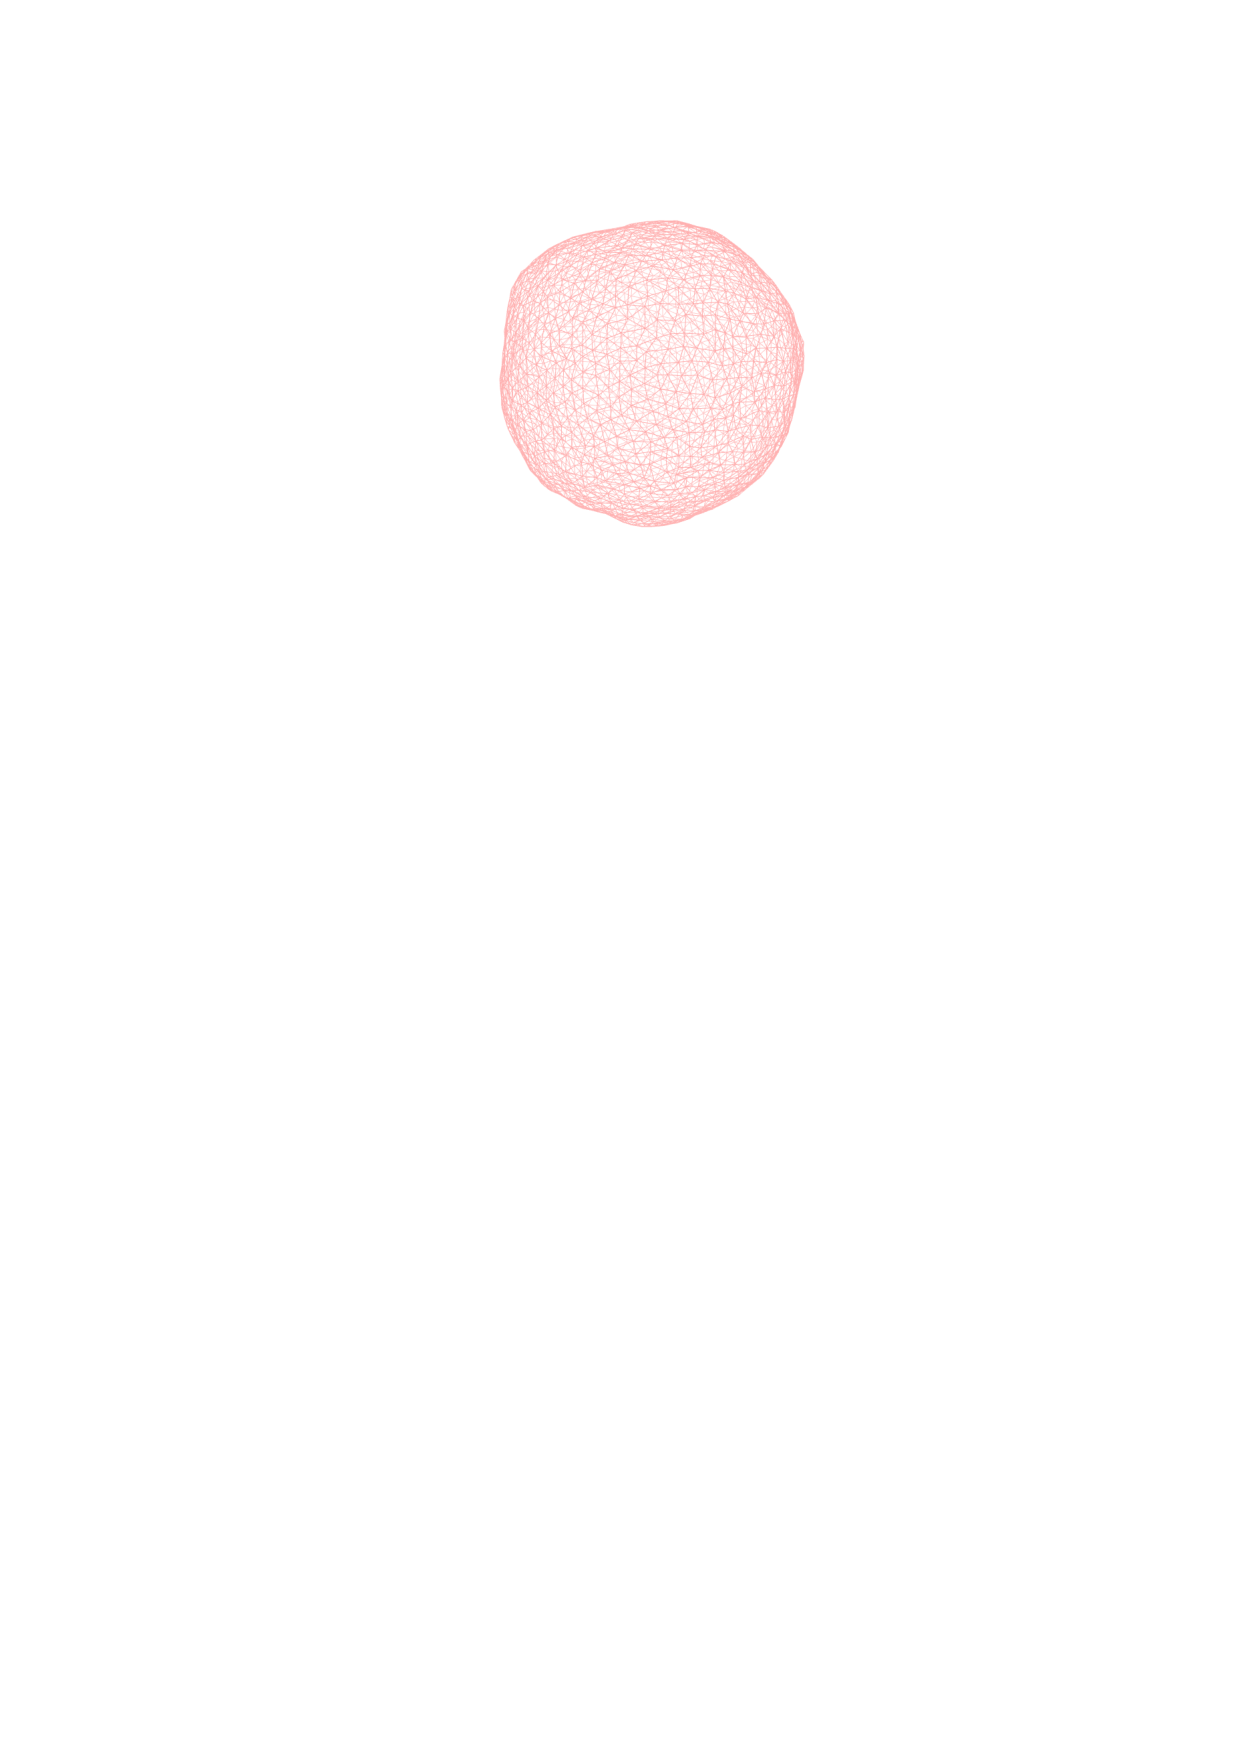
\includegraphics[width=4in]{mem_sim1}
\caption{
غشا با هندسه‌ی کروی.
}
\label{fig:mem1}
\end{center}
\end{figure}
\begin{figure}[h]
\begin{center}
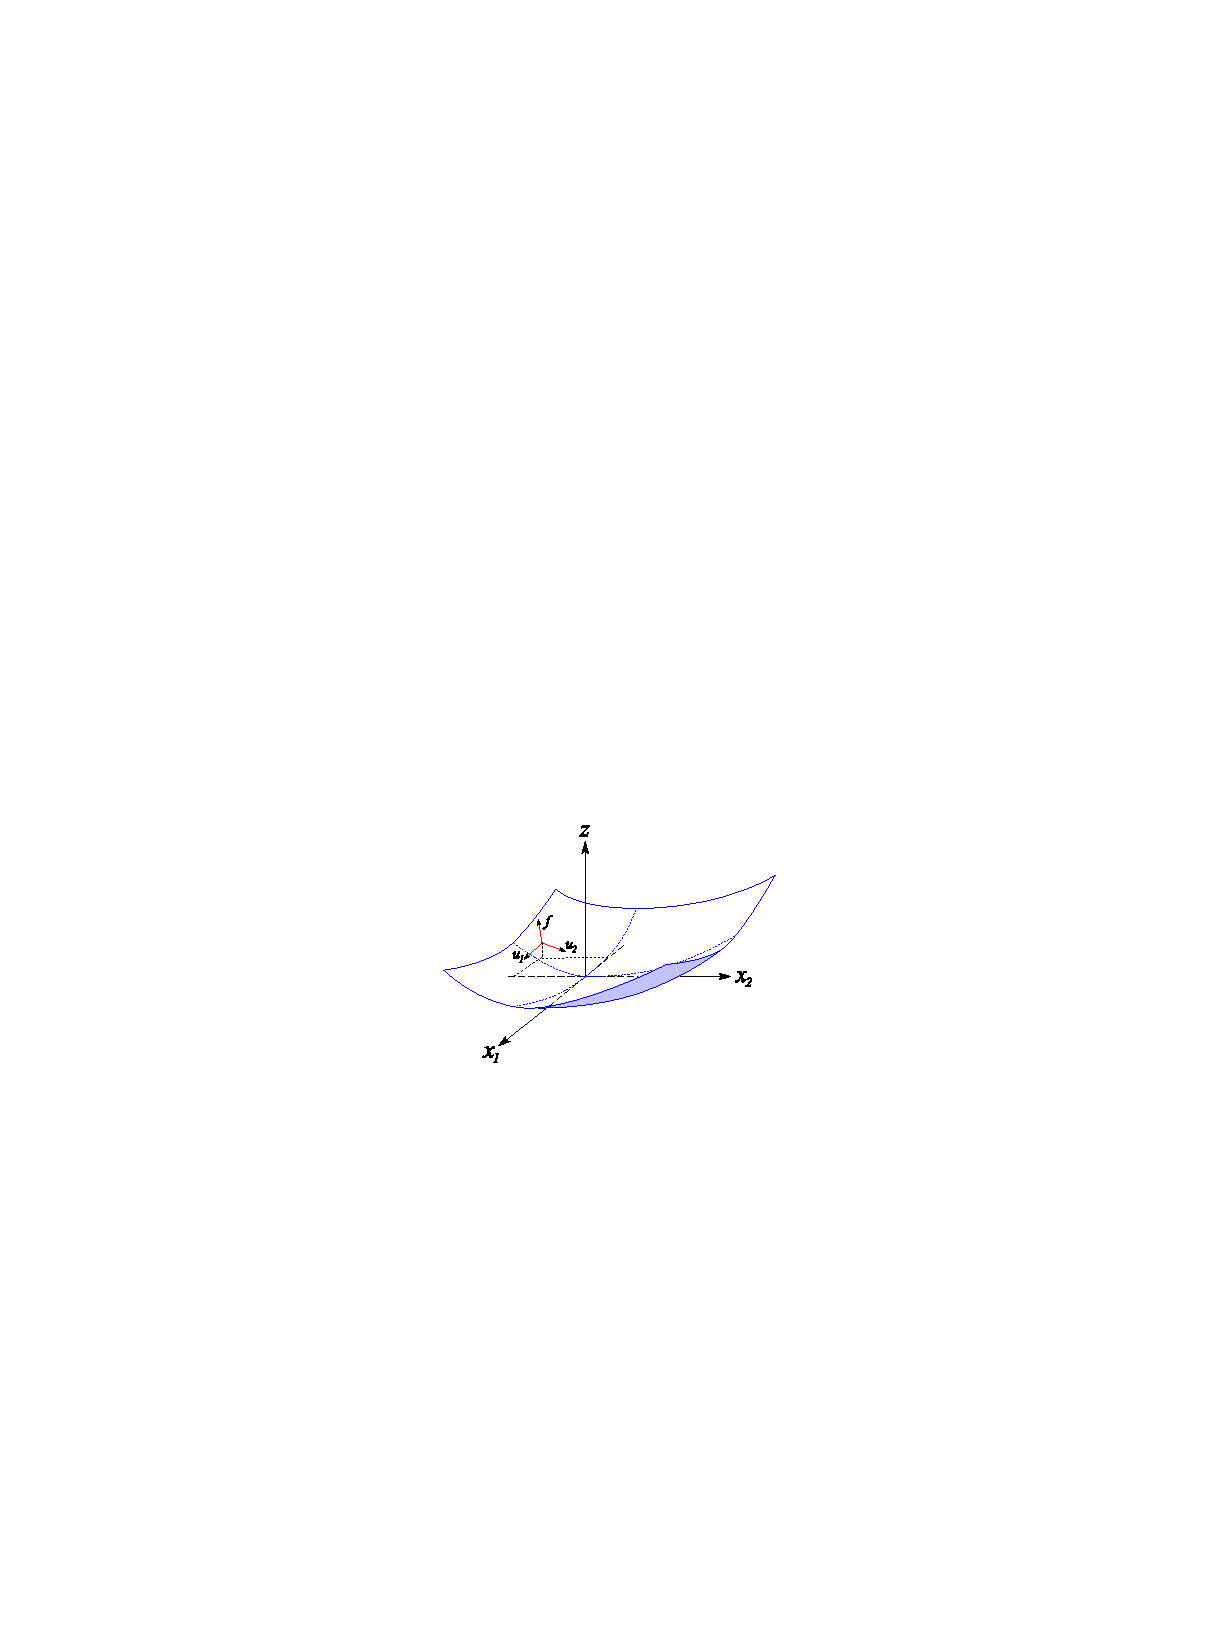
\includegraphics[width=4in]{nelsonS1}
\caption{
مبدا مختصات مماس به بخشی از کره‌ی بدون تغییر شکل.ٓ
}
\label{fig:nelson_figs1}
\end{center}
\end{figure}

که در اینجا 
$z=Z()z_1,x_2)$
نقاط روی کره در حالت بدون اختلال را مشخص می‌کند. در نظریه پوسته‌ی کم عمق فرض می‌شود که محل بررسی به اندازه‌ای کوچک است که شیب‌های 
$\partial_1Z\sim x_1/R$
و 
$\partial_2Z\sim x_2/R$
اندازه‌گیری شده نسبت به صفحه‌ی 
$(x_1,x_2)$
کوچک هستند. در نتیجه می‌توان معادله‌ی بالا رو به شکل زیر ساده کرد:
\begin{equation}
Z(x_1,x_2) \approx \frac{x_1^2+x_2^2}{2R}
\label{eq:nelsonS2}
\end{equation}
در نتیجه تمام تغییر شکل‌های پوسته از این حالت را می‌توان بر حسب جابجایی‌های عمود بر صفحه‌
 $f(x_1,x_2)$
و جابجایی های مماس بر صفحه 
$u_1(x_1,x_2)$
و
$u_2(x_1,x_2)$
که به ترتیب جابجایی در راستای محورهای 
$x_1$
و
$x_2$
را مشخص می‌کنند، تعریف کرد. بنابراین با توجه به میدان‌های تعریف شده، نقطه‌ی 
$(x_1,x_2,Z(x_1,x_2))$
در حالت بدون جابجایی در مرتبه‌ی اول به نقطه‌ی 
$(x_1+u_1-f\partial_1Z,x_2+u_2-f\partial_2Z,Z+f)$
منتقل می‌شود که در اینجا 
$\partial_iZ=x_i/R$
است. تانسور کرنش با توجه رابطه‌ی میان اندازه‌ی یک عنصر خط در حالت تغییر حالت داده شده
$ds'$
و خط متناظر آن در حالت کاملا کروی تعریف می‌شود:
\begin{equation}
(ds')^2=ds^2+2u_{ij}dx_idx_j
\label{eq:nelsonS3}
\end{equation}
در نتیجه با صرف نظر از مشتق‌های مرتبه‌های بالاتر می‌توان تانسور کرنش را تعریف کرد،
\begin{equation}
u_{ij}=\frac{1}{2}(\partial_iu_j+\partial_ju_i+\partial_if\partial_jf)-\delta_{ij}\frac{f}{R}
\label{eq:nelsonS4}
\end{equation}
در نتیجه انرژی کششی به شکل زیر تعریف خواهد شد
\begin{equation}
G_s=\frac{1}{2}\int dS\left[2\mu u_{ij}^2+\lambda u_{kk}^2\right]
\label{eq:nelsonS5}
\end{equation}
  که در اینجا 
$\lambda$
و
$\mu$
ضرایب لامه
\LTRfootnote{Lamé}
بوده و 
$dS$
عنصر مساحت است. همچنین انرژی هلفریش
\LTRfootnote{Helfrish}
را نیز در برای تغییرات خمشی پوسته در نظر می‌گیریم
\cite{Helfrich1973}.
\begin{equation}
G_b=\frac{1}{2}\int dS\left[\kappa(H-H_0)^2+\bar\kappa K\right]
\label{eq:nelsonS6}
\end{equation}
  که در اینجا 
$\kappa$
سختی خمشی، 
$H$
خمش متوسط (یا رد
\LTRfootnote{trace}
تانسور خمش)،
$H_0$
خمش ذاتی غشا،
$\bar\kappa$
مدول خمشی زینی،
و
$K$
دترمینان تانسور خمش است . با توجه به نظریه گاوس و بونه
\LTRfootnote{Gauss-Bonnet}
این انتگرال فقط یک عدد ثابت است که به انرژی آزاد سیستم اضافه می‌شود. در نتیجه از الان به بعد آن را در نظر نمی‌گیریم. همچنین فرض می‌کنیم که غشا خمش ذاتی ندارد. در نتیجه در قسمت کم عمق پوسته خمش موضعی بر حسب 
$Z(x_1,x_2)$
و 
$f(x_1,x_2)$
به شکل زیر محاسبه می‌شود:
\cite{Helfrich1973}.
\begin{equation}
H =\nabla^2(Z+f)=\frac{2}{R}+\nabla^2f
\label{eq:nelsonS7}
\end{equation}
که 
$\nabla^2=\partial_{11}+\partial_{22}$
لاپلاسین در دستگاه مختصات تعریف شده است. و در نهایت کار ناشی از فشار خارجی به صورت زیر تعریف می‌شود،
\cite{Helfrich1973}.
\begin{equation}
W=-p\int dSf
\label{eq:nelsonS8}
\end{equation}

و در نهایت  عنصر سطح به شکل زیر تعریف می‌شود،
\begin{equation}
dS=dx_1dx_2/\sqrt{1-(x_1^2+x_2^2)/R^2}\approx dx_1dx_2
\label{eq:nelsonS8.1}
\end{equation}
در نهایت با جمع کردن جملات انرژی کششی، خمشی، و فشار انرژی کشسانی سیستم به شکل زیر تغریف می‌شود:
\begin{equation}
G = G_s + G_b. + W =\int d^2x\left[\frac{\kappa}{2}(\nabla^2f)^2+\mu u_{ij}^2+\lambda u_{kk}^2-pf\right]
\label{eq:nelsonS8.2}
\end{equation}
همانطور که از نام این نظریه پیداست مدل بالا برای محاسبه‌ی انرژی لازم برای تغییر شکل‌ها کم عمق و کوچک است. مقیاس ما از اندازه‌ی کره شعاع آن
$R$
است. حد اندازه‌ی یک تغییر شکل کوچک را می‌توانیم با مقایسه‌ی انرژی کششی و خمشی محاسبه کنیم. انرژی کششی و خمشی برای قسمتی به اندازه‌ی
$\ell$
را با 
$G_s\sim Y(f/R)^2$
، که در اینجا $Y$ یک ثابت کششی‌ متداول است، و 
$G_b\sim\kappa f^2/\ell^4$
می‌توان تقریب زد. برابر قرار دادن این دو جمله، مقیاس طولی فوپل فون کارمان
\LTRfootnote{Föpplٓ-von Kármán}
را به ما می‌دهد
\begin{equation}
\ell^*=\frac{R}{\gamma^{1/4}}
\label{eq:nelsonS9}
\end{equation}
که در بالا عدد فوپل فون کارمان 
$\gamma=YR^2/\kappa$
است
\cite{nelsonPRE2003}
. با کمی محاسبه‌ی بیشتر می‌توان نشان داد که ثابت کششی که استفاده کردیم مدول ۲ بعدی یانگ است که برابر است با 
\begin{equation}
Y= \frac{4\mu(\mu+\lambda)}{2\mu+\lambda}
\label{eq:nelsonS9.1}
\end{equation}
با فرض داشتن یک پوسته‌ی کشسان با ضخامت $h$ و جایگذاری $\kappa$ و $Y$ با مدول ۳ بعدی یانگ برای یک ماده جامد همسان کشسان در نظریه پوسته‌ی کم عمق $\gamma\approx10(R/h)^2$ بدست می‌آید 
\cite{landau}
برای اینکه این نظریه پیشبینی درستی از مسئله داشته باشد نیاز است که $\ell^*\ll R$. پس این نظریه تنها زمانی که $\gamma\gg1$ یا $r\gg h$ باشد صادق است که این حد دقیقا متناظر با پوسته‌های نازکی است که می‌توانند تحت تاثیر بسیار زیاد افت و خیز ترمودینامیکی قرار بگیرند. کویتر
\LTRfootnote{Koiter}
در مطالعاتی نیز در مورد صحت پاسخ نظریه‌ی پوسته‌های کم عمق در مقایسه با نظریه‌های عمومی‌تر که می‌توان بر تمامی یک پوسته‌ی کشسان اعمال کرد را در حالتی که از دو نقطه‌ی قطبی به یک پوسته فشار وارد می‌شود بحث کرده است
\cite{koiter1963}
 . همچنین توسط هاتچینسون
\LTRfootnote{Hutchinson}
برای مطالعه‌ی پایداری پوسته‌های تحت فشار مطالعه شده‌است
\cite{Hutchinson1967}
. در هر دو مطالعه نشان داده شده که این نظریه در مقیاسی که در بالا محاسبه کردیم رفتار درستی از سیستم را نشان می‌دهد. از آنجایی که افت و خیز گرمایی روی پوسته‌هایی که شعاع آنها بسیار بزرگ‌تر از زخامتشان است تاثیر زیادی‌ می‌گذارد، این نظریه را می‌توان به عنوان نقطه‌ شروع توصیف این سیستم‌ها استفاده کرد.
\subsection{
از میان رفتن مُدهای فنونی درون صفحه‌ای و انقباض هماهنگ کروی بوسیله‌ی انتگرال گاووسی
}
\LTRfootnote{Elimination of in-Plane Phonon Modes and Uniform Spherical Contrac- tion by Gaussian Integration}
یک پوسته‌ی کروی تحت فشار هماهنگ خارجی که از حد مچاله شدن کره
\LTRfootnote{buckling}
کمتر است باعث می‌شود که کره در تمام نقاط به صورت هماهنگ به اندازه‌ی $f_0$ منقبض شود. در نتیجه‌ تغییر شکل‌های خارج از صفحه‌ای را می‌توان به صورت مجموع قسمت‌های هماهنگ و غیر هماهنگ نوشت،
\begin{equation}
f(\boldsymbol x)=f_0+f'(\boldsymbol x) = f_0+\sum_{\boldsymbol . q\neq0}f_{\boldsymbol q}e^{-i\boldsymbol q.\boldsymbol x}
\label{eq:nelsonS10}
\end{equation}
در اینجا $f'(\boldsymbol x)$ 
نماینده‌ی سهم میدان از مد‌های غیر صفر مولفه‌های فوریه‌ی آن است. در این بخش برای ساده سازی از نرمال کردن 
$f_{\boldsymbol q} \equiv \frac{1}{A}\int d^2xf(\boldsymbol x) e^{i\boldsymbol q.\boldsymbol x}$
استفاده شده که $A$ مساحت انتگرال گیری شده روی صفحه‌ی $(x_1,x_2)$ است. همچنین تبدیل واروون را نیز به شکل 
$f(\boldsymbol x) = \sum_{\boldsymbol q}f_{\boldsymbol q}e^{-i\boldsymbol q.\boldsymbol x}$
در این صورت 
$\int d^2xf'(\boldsymbol x)=0$
است و در نتیجه تنها جمله‌‌ی $f_0$ در محاسبه‌ی کار فشار باقی می‌ماند. از آنجایی که جمله‌ی $f'$ تنها در قسمت غیر خطی تانسور کرنش ظاهر می‌شود، پس انرژی کشسانی که در معادله‌ی \ref{eq:nelsonS8.2} تعریف شد در حالت انقباض تحت فشار هماهنگ $f_0$ و همچنین تحت جابجایی مُدهای درون صفحه‌ای $u_1(\boldsymbol x)$ و $u_2(\boldsymbol x)$ به شکل همسان
\LTRfootnote{harmonic}
 عمل می‌کند. برای بررسی رفتارهای غیر همسان بهتر است که این میدان‌ها را تقریب بزنیم و از انرژی آزاد مؤثر تعریف کنیم.
 \begin{equation}
G_{eff}=-k_BT\ln\left\{\int\mathcal D\vec u(x_1,x_2)\int df_0e^{-G[f',f_0,u_1,u_2]/k_BT}\right\}
\label{eq:nelsonS11}
\end{equation}
برای اینکه انتگرال تابعی را در معادله‌ی بالا را برای تعداد مشخصی میدان جابجایی خارج از صفحه‌ای $f'(\boldsymbol x)$ بتوانیم انجام دهیم باید جملات $\boldsymbol q = 0$ و $\boldsymbol q \neq 0$ تانسور کرنش $u_{ij}$ 
را نیز از هم جدا کنیم،

 \begin{equation}
u_{ij}=\tilde u_{ij}^0+\sum_{\boldsymbol q \neq 0}\left[\frac{i}{2}\left(q_iu_j(\boldsymbol q)+q_ju_i(\boldsymbol(q)\right)+A_{ij}(\boldsymbol q)-\delta{ij}\frac{f_{\boldsymbol q}}{R}\right]e^{-i\boldsymbol q.\boldsymbol x}
\label{eq:nelsonS12}
\end{equation}
که در بالا 
 \begin{equation}
A_{ij}(\boldsymbol q)=\frac{1}{2A}\int d^2x\partial_if'\partial_jf'e^{i\boldsymbol q.\boldsymbol x}
\label{eq:nelsonS13}
\end{equation}
قسمت هماهنگ تانسور کرنش از اجزای زیر تشکیل شده
\begin{equation}
\begin{aligned}
&\tilde u_{11}^0=u_{11}^0+A_{11}(\boldsymbol 0)-\frac{f_0}{R}, \\
&\tilde u_{22}^0=u_{22}^0+A_{22}(\boldsymbol 0)-\frac{f_0}{R}, \\
&\tilde u_{12}^0=u_{12}^0+A_{12}(\boldsymbol 0)
\label{eq:nelsonS14}
\end{aligned}
\end{equation}
در بالا $u_{ij}^0$ جملات کرنشی هماهنگ درون صفحه‌ای مستقل از $f_0$. این محدودیت باعث می‌شود که $u_{11}^0+u_{22}^0=0$ باشد زیرا اگر تغییر شکل هم علامت در راستای $x_1$ و $x_2$ در پوسته وجود داشته باشد به این معناست که شعاع پوسته در حال تغییر کردن است که تغییرات این چنین در  جمله‌ی $f_0$ در نظر گرفته شده است. در نتیجه علاوه بر $f_0$
و $u_{12}^0$
تنها یک درجه‌ی آزادی مستقل دیگر وجود دارد که در تانسور کرنش تاثیر هماهنگ دارد و آن $\Delta u^0 = u_{11}^0-u_{22}^0$ است.
در نهایت لازم است که انتگرال تابعی در معادله \ref{eq:nelsonS11} را روی میدان‌های فنونی $u_i$ 
و ۳ درجه‌ی آزادی مستقل که سهم جملات هماهنگ در تانسور کرنش دارند، 
$f_0$، $\tilde u_{12}^0$، و$\Delta u^0$
را حساب کنیم. پس از حذف جملاتی که به صورت عدد ثابل ظاهر می‌شوند انرژی آزاد مؤثر شکل زیر را به خود می‌‌گیرد،
ٓ\begin{equation}
G_{eff}=\int d^2x\left[\frac{\kappa}{2}(\nabla^2f')^2+\frac{Y}{2}\left(\frac{1}{2}P_{ij}^T\partial_if'\partial_jf'-\frac{f'}{R}\right)\right]-A\frac{pR}{2}[A_{11}(\boldsymbol 0)+A_{22}(\boldsymbol 0)]
\label{eq:nelsonS15}
\end{equation}
که در بالا $P_{ij}^T=\delta_{ij}-\partial_i\partial_j/\nabla^2$ عملگر تصویری عرضی‌ است
\LTRfootnote{transverse projection operator}
. توجه کنید که در نتیجه‌ی انتگرال گیری، مؤلفه‌های لامه $\mu$ و $\lambda$ فقط از طریق مدول ۲ بعدی یانگ وارد می‌شوند. در آخر با جایگذاری
\begin{equation}
A_{11}(\boldsymbol 0)+A_{22}(\boldsymbol 0)=\frac{1}{2A}\int d^2x\left[ (\partial_1f')^2+(\partial_2f')^2\right] = \frac{1}{2A}\int d^2x| \nabla f'|^2
\label{eq:nelsonS16}
\end{equation}
در معادله‌‌ی \ref{eq:nelsonS15} 
انرژی آزاد مؤثر $G_{eff}$ دو بخش هماهنگ $G_0$ 
و غیر هماهنگ $G_1$
خواهد داشت،
\begin{equation}
\begin{aligned}
&G_0=\frac{1}{2}\int d^2x\left[\kappa(\nabla^2f')^2-\frac{pR}{2}|\nabla f'|^2+\frac{Y}{R^2}f'^2\right], \\
&G_1=\frac{Y}{2}\int d^2x\left[\left(\frac{1}{2}P_{ij}^T\partial_if'\partial_jf'\right)^2-\frac{f'}{R}P_{ij}^T\partial_if'\partial_jf'\right],
\label{eq:nelsonS16.1}
\end{aligned}
\end{equation}
در معادله‌ی بالا $Y=4\mu(\mu+\lambda)/(2\mu+\lambda)$ مدول یانگ در ۲ بعد است. جمله‌ی «جرم» $Y(f'/R)^2$ در تابعی انرژی هماهنگ میزان جفت شدگی بین تغییر شکل خارج از صفحه و کشیدگیی که درون صفحه ایجاد می‌شود را مشخص می‌کند. این جمله در نظریه‌ی صفحات یا غشاهای تخت ظاهر نمی‌شود. همچنین برهمکنشی با ضریب $-Y/2R$ نیز جمله‌ایست که مخصوص غشاهای خمیده‌است و به علت وجود تقارن در غشاهای تخت دیده نمی‌شود. نکته جالب راجع به این جملات این است که در آنها پارامترهای وابسته به اندازه سیستم در آنها وجود دارد. توجه داشته باشید که برای فشارهای رو به داخل $p>0$ در قسمت هماهنگ معادله شبیه کشش سطحی منفی و وابسته به شعاع رفتار می‌کند. در حد $R\rightarrow \infty$ و $p=0$ انرژی غشای تخت بدست می‌آید. از آنجایی که $f_0$ 
پس از انتگرال گیری ظاهر نمی‌شود و از این پس به جای 
$f'$ از 
$f$ 
استفاده خواهیم کرد. اگر تنها اثر جملات هماهنگ را درنظر بگیریم، نتایج بر اساس اصل همپاری برای مؤلفه‌های فوریه ناشی از گرما برای موج ۲ بعدی

\begin{equation}
\begin{aligned}
&f_{\boldsymbol q} = \int d^2xf(\boldsymbol x)e^{i\boldsymbol q.\boldsymbol x}, \\
&\left\langle f_{\boldsymbol q}f_{\boldsymbol {q'}}\right\rangle_0 = \frac{Ak_BT\delta_{\boldsymbol q, \boldsymbol{-q'}}}{\kappa q^4-\frac{pR}{2}q^2+\frac{Y}{R^2}},
\label{eq:nelsonS17}
\end{aligned}
\end{equation}
که در بالا $A$
مساحت قسمت انتگرال گیری است. 
بزرگی طول موج‌ها بلند به علت اندازه محدود کره به $q\gtrsim 1/R$
محدود می‌شوند. برخلاف غشاهای تخت که طول موج‌های بلند $q\rightarrow 0$
با اهنگ $k_BT/(\kappa q^4)$
به بینهایت میل می‌کند، در غشاهای خمیده جفت شدگی میان خمیدگی خارج از صفحه و درون صفحه، طول موج افت و خیزها با سقف مشخصه‌ی طول سیستم محدود می‌شوند، 
\begin{equation}
q^*=(\ell^*)^{-1}=\left(\frac{Y}{\kappa R^2}\right)^{1/4}\equiv\frac{\gamma^{1/4}}{R}
\label{eq:nelsonS17.1}
\end{equation}
که ما در اینجا حالت‌های $\gamma\gg1$
که در نتیجه $\ell^*\ll R$
را بررسی می‌کنیم. در حالی که $p$
به $p_c\equiv4\sqrt{\kappa Y}/R^2$
نزدیک می‌شود،. طول موج‌های $q=q^*$ 
ناپایدار شده و اندازه‌ی آنها به بی‌نهایت می‌رود. در نتیجه این حالت معادل با مچاله شدن پوسته‌ی کروی تحت فشارهای خارجی بالاتر از حد تحمل سیستم است. برای فشارهای بیشتر از $p_c$
نمی‌توانیم از این نظریه استفاده کنیم زیرا که تغییرات در شکل کره فراتر از تغییرات کم عمق خواهد بود.

معادله‌ی \ref{eq:nelsonS17}
 رفتار هماهنگ پوسته‌ی کروی را بیان می‌کند، برای بررسی رفتار ناهماهنگ پوسته نیاز است که به این معادله جمله‌های تصحیح کننده اضافه کنیم.
 \subsection{محاسبه‌ی سهم تک حلقه در خود انرژی}
 \begin{figure}[h]
\begin{center}
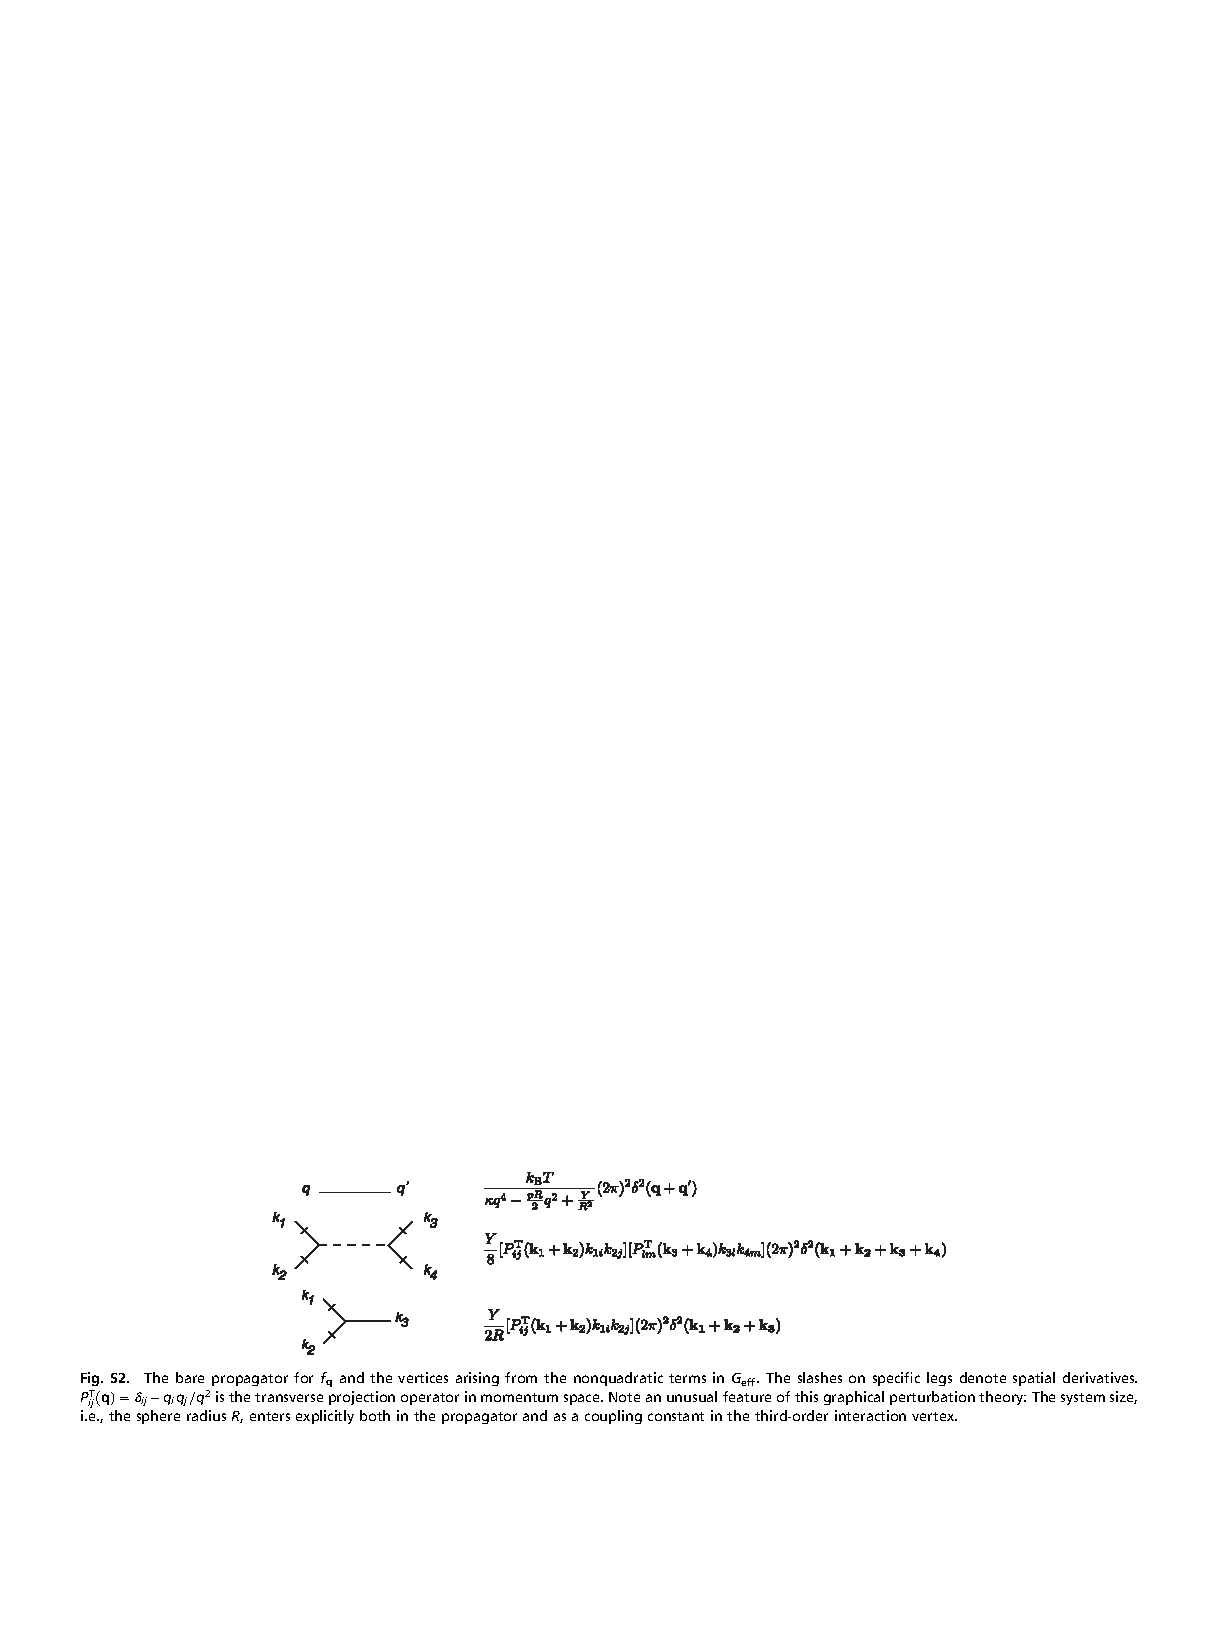
\includegraphics[width=4in]{nelsonS2}
\caption{
غشا با هندسه‌ی کروی.
}
\label{fig:nelsonS2}
\end{center}
\end{figure}

\begin{figure}[h]
\begin{center}
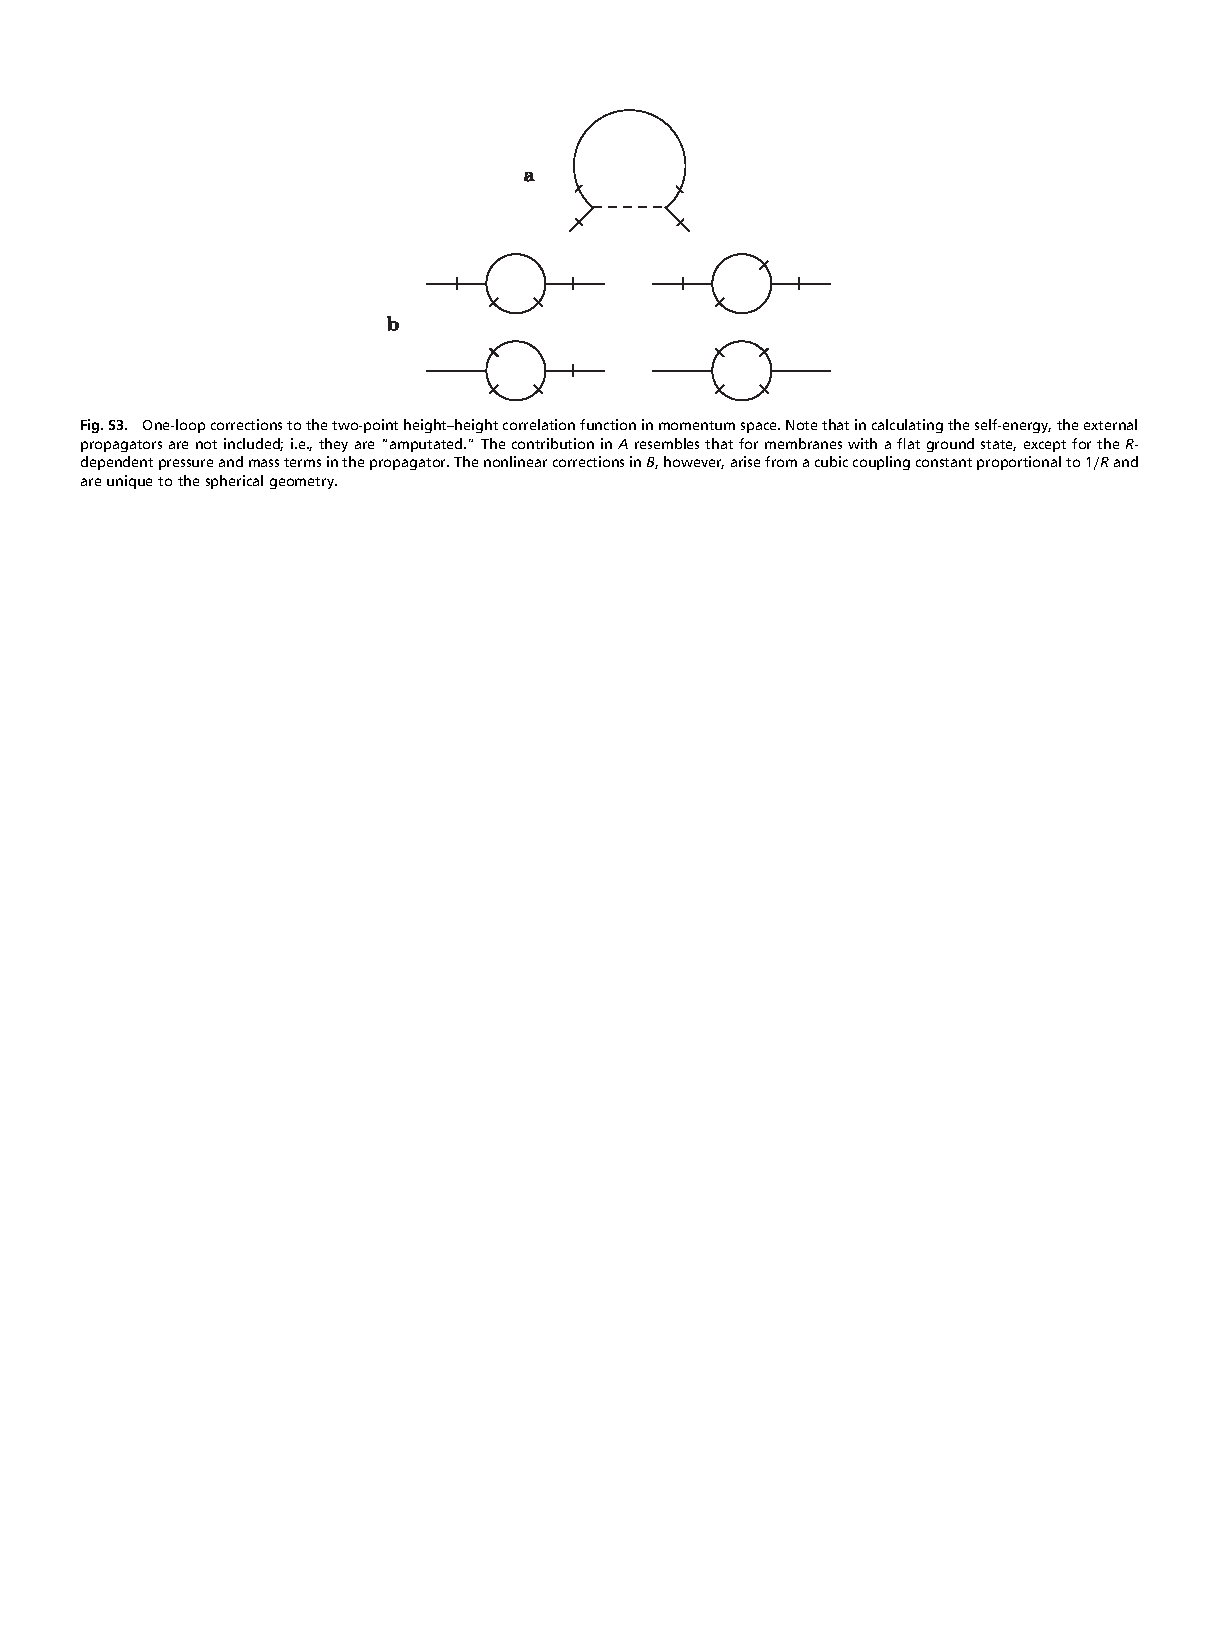
\includegraphics[width=4in]{nelsonS3}
\caption{
غشا با هندسه‌ی کروی.
}
\label{fig:nelsonS3}
\end{center}
\end{figure}
X
 قوانین فاینمن برای برگرفته شده از معادله‌ی \ref{eq:nelsonS15} 
 در شکل \ref{fig:nelsonS2}
 خلاصه شده است. از این پس مؤلفه‌های تبدیل فوریه به شکل
 $f_{\boldsymbol q}=\int d^2xf(\boldsymbol x)\exp(i\boldsymbol q.\boldsymbol x)$
 تعریف می‌شود. تبدیل فوریه‌ی وارون تغییر شکل‌های خارج از صفحه نیز به صورت
\begin{equation}
f(\boldsymbol x)=\frac{1}{A}\sum_{\boldsymbol q\neq 0}f_{\boldsymbol q}e^{-i\boldsymbol q.\boldsymbol x}
\label{eq:nelsonSٓ18}
\end{equation}
تعریف می‌شود و جمع روی تمام طول موج‌های مجاز است. خود انرژی ناشی از جمله‌ی ناهماهنگ ۳ نقطه‌ای و ۴ نقطه‌ای در شکل \ref{fig:nelsonS3}
الف خلاصه شده‌اند و این جملات برای توصیف غشای تخت نیز لازم هستند و به شکل 
\begin{equation}
-Y\int\frac{d^2k}{(2\pi)^2}\frac{\left[P_{ij}^Tq_iq_j\right]^2}{\kappa|\boldsymbol q + \boldsymbol k|^4-\frac{pR}{2}|\boldsymbol q + \boldsymbol k|^2+\frac{Y}{R^2}}
\label{eq:nelsonS19}
\end{equation}
 مجموع جملات خود انرژی ناشی از نمودارهای \ref{fig:nelsonS3}
 ب،

\begin{equation}
\begin{aligned}
&\frac{Y^2}{R^2} \int\frac{d^2k}{(2\pi)^2} \frac{1}{ 
\left( \kappa|\boldsymbol q + \boldsymbol k|^4 - \frac{pR}{2} |\boldsymbol q + \boldsymbol k|^2 + \frac{Y}{R^2} \right)
\left( \kappa k^4 - \frac{pR}{2}k^2 + \frac{Y}{R^2} \right) 
} \\
&\times\left\{ 
\frac{1}{2} \left[ P_{ij}^T(\boldsymbol q)k_ik_j\right]^2 + 
\left[P_{ij}^T(\boldsymbol k)q_iq_j\right]^2 + 
\left[P_{ij}^T(\boldsymbol k)q_iq_j\right] 
\left[P_{lm}^T(\boldsymbol{k+ q})q_lq_m\right] \right.\\
& \left.+ 2\left[P_{ij}^T(\boldsymbol k)q_iq_j\right]
\left[P_{lm}^T(\boldsymbol{q})k_lk_m\right]
\right\}
\label{eq:nelsonS20}
\end{aligned}
\end{equation}
وارون تابع همبستگی هماهنگ که در معادله‌ی \ref{eq:nelsonS17} مشاهده کردید فقط از جملات $q^0$، $q^2$، و $q^4$ تشکیل شده است و تصحیحات تک حلقه (که در معادلات \ref{eq:nelsonS19} و \ref{eq:nelsonS20} محاسبه شد) انجام شده به طیف جملاتی با همین توان‌ها و همچنین جملاتی با مرتبه‌ی $q^6$ نیز اضافه می‌کند. اگر  تصحیحات را تنها تا مرتبه‌ی $q^4$ نگه داریم می‌توانیم طیف را برای $q$های
کوچک تقریب بزنیم. 
\begin{equation}
Ak_BT\left\langle|f_{\boldsymbol q\rightarrow \boldsymbol 0}|^2\right\rangle^{-1} \equiv\kappa_Rq^4-\frac{p_RR}{2}q^2+\frac{Y_R}{R^2}+O(q^6)
\label{eq:nelsonS21}
\end{equation}
 که در بالا $Y_R$، $\kappa_R$، و $p_R$ به ترتیب مدول یانگ مؤثر، سختی خمش مؤثر، و فشار بی بعد. در مقیاس‌های طولی بزرگ اندازه‌گیری مشخصات کشسانی پوسته‌هایی که با گرما افت و خیز می‌کنند اطلاعاتی در مورد مشخصات مؤثر کشسانی در اختیار ما قرار می‌دهد. استفاده از این مشخصات بهتر از استفاده از مدول‌های خام $Y$، $\kappa$، و $p$
است که با تقریب دمای صفر رفتار پوسته در دما توصیف می‌کنند. با استفاده از معادلات \ref{eq:nelsonS19} و \ref{eq:nelsonS20} 
تا مرتبه‌ی $O(q^4)$
می‌توان انتگرال‌های تکانه را برای خود انرژی محاسبه کنیم،
\begin{equation}
Y_R=Y\left[1-\frac{3}{128\pi}\frac{k_BT}{\kappa}\frac{\sqrt\gamma}{(1-\eta^2)^{3/2}}\left(\eta\sqrt{1-\eta^2}+\pi-\cos^{-1}\eta\right)\right]
\label{eq:nelsonS22}
\end{equation}

\begin{equation}
\begin{aligned}
&\kappa_R=\kappa\left[1+\frac{1}{30720\pi}\frac{k_BT}{\kappa}\frac{\sqrt\gamma}{(1-\eta^2)^{7/2}}\right.\\
&\left.\left[\times\eta\sqrt{1-\eta^2}(-1699+3758\eta^2-2104\eta^4) \right.\right.\\
& \left.\left. +15(61-288\eta^2+416\eta^4-192\eta^6)(\pi-\cos^{-1}\eta)\right]\right]
\label{eq:nelsonS23}
\end{aligned}
\end{equation}

\begin{equation}
\begin{aligned}
&\eta_R=\eta+\frac{1}{1536\pi}\frac{k_BT}{\kappa}\frac{\sqrt\gamma}{(1-\eta^2)^{5/2}}\\
&\times\left[\sqrt{1-\eta^2}(64-67\eta^2)+3(21\eta-22\eta^3)(\pi-\cos^{-1}\eta)\right]
\label{eq:nelsonS24}
\end{aligned}
\end{equation} 
و در معادلات بالا فشار بی بعد $\eta=p/p_c$
تعریف کردیم. به طور مشخص زمانی که $\eta\rightarrow1$
این کمیت‌ها به بی‌نهایت میل می‌کنند. این جملات برای پایین‌ترین مرتبه فشار خارجی به شکل زیر تقریب زده می‌شوند،
 \begin{equation}
Y_R\approx Y\left[1-\frac{3}{256}\frac{k_BT}{\kappa}\sqrt\gamma\left(1+\frac{4}{\pi}\frac{p}{p_c}\right)\right]
\label{eq:nelsonS25}
\end{equation}

\begin{equation}
p_R\approx p+\frac{1}{24}\frac{k_BT}{\kappa}p_c\sqrt\gamma\left(1+\frac{63\pi}{128}\frac{p}{p_c}\right)
\label{eq:nelsonS26}
\end{equation}

\begin{equation}
\kappa_R\approx \kappa\left[1+\frac{61}{4096}\frac{k_BT}{\kappa}\sqrt\gamma\left(1-\frac{1568}{915\pi}\frac{p}{p_c}\right)\right]
\label{eq:nelsonS27}
\end{equation}
برای محاسبه‌ی انتگرال‌های بالا باید از انتگرال‌های معادلات \ref{eq:nelsonS19} و \ref{eq:nelsonS20} روی تمام طول‌ موج‌های مجاز فضای فاز انتگرال بگیریم. طول‌ موج‌ها از حد پایین $k_{min}\sim1/R$ تا حد بالای طول موج‌ که با ثابت میکروسکوپیک شبکه‌ی شبکه تعیین می‌شود، است. از آنجایی که تمام انتگرال‌ها در حد بالا به حد فرابنفش همگرا می‌شوند می‌ توانیم $k\rightarrow\infty$. به علت وجود جمله‌ی «جرم» $\sim Y/R^2$ انتگرال در محدوده‌ی طول موج‌های کوچک خوش رفتار است، و در نتیجه می‌توان انتگرال را در این محدوده روی تمام فضای فاز دو بعدی انجام دهیم. اینکه انتگرال را برای محدوده‌ی پایین‌تر از فروسرخ یا $0<k<1/R$ انجام دهیم باعث ایجاد خطای از مرتبه‌ی $1/\sqrt\gamma$ می‌شود که برای پوسته‌های خیلی نازک قابل صرف نظر کردن است. 

با نگاه کردن به معادلات $\ref{eq:nelsonS25}، $\ref{eq:nelsonS26}، و \ref{eq:nelsonS27} می‌بینیم که در حد طول موج‌های بلند تغییر شکل‌های تابع مدول یانگ موثر کوچکتر، سختی خمش مؤثر بزرگتر، و کشش سطحی غیر صفر منفی است. این رفتار حتی وقتی که فشار خارجی صفر باشد نیز صادق است. وقتی $p/p_c$ بزرگ باشد، مدول یانگ و سختی خمش از تقریب دمای صفر کوچکتر می‌شوند و اندازه‌ی کشش سطحی مؤثر منفی که با $p_c$ تعیین می‌شود بسیار بزرگ می‌شود. محاسبات خطاهای مرتبه‌های بالاتر همگی نشان می‌دهند که با $p/p_c\rightarrow1$ تمام تصحیحات به بی‌نهایت میل می‌کنند. همچنین مشا‌هده می‌کنیم که تمام مشخصات مؤثر تابع دما و اندازه‌ی سیستم هستند زیرا که $\sqrt\gamma\sim R$ . با اینکه برای $k_BT\ll\kappa$ 
سهم تصحیحات ناچیز است ولی باید در نظر بگیریم که با بزرگ شدن شعاع سیستم $R\rightarrow\infty$ 
به بینهایت میل می‌کند. 


کشش سطحی ناشی از افت و خیز گرمایی و تابعیت قوی آن با فشار خارجی، همچنین تابعید ثابت کشسانی سیستم با اندازه‌ی سیستم مشخصات مختص غشاهای کروی است و در غشا‌های تخت دیده نمی‌شود. 
\subsection{بررسی با استفاده از هماهنگ‌های کروی}
یک پوسته‌ی کروی با شعاع $R$، سختی خمش $\kappa$ و مؤلفه‌های لامه $\mu$ و $\lambda$ 
در نظر بگیرید که تحت یک میدان مماسی $\boldsymbol u(u_x,u_y)$
و میدان جابجایی شعاعی $f$
قرار گرفته‌است. میدان $\boldsymbol u$
را مانند تمام میدان‌های خوش رفتار می‌توان مجموع یک بخش بدون چرخش
\LTRfootnote{curl free}
و بخش بدون واگرایی
\LTRfootnote{divergence free}
نوشت، $\boldsymbol u\equiv\nabla\boldsymbol\Psi+\boldsymbol v$ که تابع اسکالر $\boldsymbol\Psi$ قسمت غیرچرخش
\LTRfootnote{irrotational}
 را تولید می‌کند و $\boldsymbol v$ بخش مارپیچی
 \LTRfootnote{solenoidal}
 است. در بخش شعاعی مختصات شعاعی نود $i$ 
 در مختصات زاویه‌ای $(\theta,\phi)$ را می‌توانیم به شکل $r_i(\theta,\phi)=R_0+f(\theta,\phi)$
 نوشت و $R_0$ در اینجا شعاع متوسط کره‌ی در حال افت و خیز است.
 هنگام بسط دادن بر حسب هماهنگ‌ها کروی حقیقی به شکل
\begin{equation}
\begin{aligned}
&f(\theta,\phi)=R\sum_{l=0}^{l_M}\sum_{m=-l}^{m=l}A_{lm}Y_{lm}(\theta,\phi)\\
&\boldsymbol\Psi(\theta,\phi)=R^2\sum_{l=0}^{l_M}\sum_{m=-l}^{m=l}B_{lm}Y_l^m(\theta,\phi)
\label{eq:nelsonS28.1}
\end{aligned}
\end{equation} 

خواهند بود و انرژی کشسانی تغییر شکل آن تا مرتبه‌ی دوم تحت این میدان‌ها طبق معادله‌ی زیر خواهد بود \cite{krollPRE1993}

\begin{equation}
\begin{aligned}
&G=R^2\sum_{l,m}\left\{\left[\frac{\kappa}{2}\frac{(l+2)^2(l-1)^2}{R^2}+2K\right]A_{lm}^2-2Kl(l+1)A_{lm}B_lm\right.\\
&\left.+\frac{1}{2}l(l+1)[(K+\mu)l(l+1)-2\mu]B_{lm}^2\right\}+G_{sol}(\boldsymbol v)
\label{eq:nelsonS28}
\end{aligned}
\end{equation} 
که در اینجا $K=\mu+\lambda$
برابر مدول حجمی‌ 
\LTRfootnote{bulk modulus}
است. قسمت مارپیچی باعث انرژی در جابجایی شعاعی نشده و انرژی جداگانه با تابعیت $\boldsymbol v$ با تابعیت مربعی دارد. همچنین به معادله‌ی بالا انرژی ناشی از کشش سطحی منفی $-pR/2$ که در اثر انقباض ناشی از وجود فشار خارجی بوجود می‌آید را به صورت $G_s=-(pR/2)\Delta A$ اضافه می‌کنیم. در اینجا $\Delta A$ سطحی مضاعفی است که به علت تغییر شکل نسبت به شعاع میانگین ایجاد می‌شود. می‌توان میزان سطح مضاعف را بر حسب هماهنگ‌های کروی نوشت.
\cite{milnersafranPRA1987}
\begin{equation}
\Delta A\approx R^2\sum_{l>1,m}A_{lm}^2\left[1+\frac{l(l+1)}{2}\right]
\label{eq:nelsonS29}
\end{equation} 
همانند تقریب انرژی کشسانی پوسته‌های کم عمق اینجا نیز روی جملات مرتبه‌ی دوم $B_{lm}$ و $\boldsymbol v$ انتگرال می‌گیریم و انرژی آزاد مؤثر سیستم را بر حسب جابجایی شعاعی می‌نوسیم،
\begin{equation}
\begin{aligned}
&G_{eff}=\frac{R^2}{2}\sum_{l>1,m}\left\{\frac{\kappa(l+2)^2(l-1)^2}{R^2}-pR\left[1+\frac{l(l+1)}{2}\right]\right.\\
&\left.+\frac{4\mu(\mu+\lambda)(l^2+l-2)}{(2\mu+\lambda)(l^2+l)-2\mu}\right\}A_{lm}^2
\label{eq:nelsonS30}
\end{aligned}
\end{equation} 
 با توجه به نظریه هم پاری انرژی،
\begin{equation}
\begin{aligned}
&k_BT\left\langle|A_{lm}|^2\right\rangle_0^{-1}\\
&=\kappa(l+2)^2(l-1)^2-pR^3\left[1+\frac{l(l+1)}{2}\right]+\frac{4\mu(\mu+\lambda)(l^2+l+2)}{(2\mu+\lambda)(l^2+l)-2\mu}R^2\\
&=\kappa(l+2)^2(l-1)^2-pR^3\left[1+\frac{l(l+1)}{2}\right]+\frac{Y}{1+\frac{Y}{2\mu(l^2+l-2)}}R^2
\label{eq:nelsonS31}
\end{aligned}
\end{equation} 
که $Y$ مدول یانگ ۲ بعدی است که قبل‌تر تعریف کردیم. حالا می‌توانیم با استفاده از پارامتر‌های وابسته به دمای مؤثر $Y_R$، $\kappa_R$، و $p_R$ به جای پارامتر‌های پایه‌ای تغییرات در افت خیز ناشی از گرما را تعریف کرد. ولی برای محاسبه‌ی آخرین جمله در معادله‌ی \ref{eq:nelsonS31} 
نیاز داریم تصحیحات گرمایی وارد بر مؤلفه‌های لامه $\mu$
و $\lambda$ 
را بدانیم. در محاسبات مربوط به نظریه‌ی پوسته‌های کم عمق این مؤلفه‌ها در محاسبات نهایی حذف شدند. در شبیه‌سازی که در مطالعه‌ی 
\cite{gomppernelson2012}
برای انرژی کشسانی گسسته‌سازی شده $\mu=3Y/8$
محاسبه شده. اگر فرض کنیم که تصحیحات گرمایی ناشی از مرتبه‌ی تک حلقه ناچیز است می‌توانیم فرض کنیم که $Y_R\approx Y$ 
است. با جایگذاری در معدله‌ی \ref{eq:nelsonS31} به همراه پارمتر‌های مؤثر دیگر به شکل نهایی زیر می‌رسیم،
\begin{equation}
\begin{aligned}
&k_BT\left\langle|A_{lm}|^2\right\rangle^{-1}\\
&\approx\kappa_R(l+2)^2(l-1)^2-p_RR^3\left[1+\frac{l(l+1)}{2}\right]+Y_RR^2\left[\frac{3(l^2+l-2)}{3(l^2+l)-2}\right]
\label{eq:nelsonS32}
\end{aligned}
\end{equation} 
حتی اگر تصحیحات گرمایی وارد بر $\mu$
و $Y$
از مرتبه‌ی $O(k_BT)$ 
باشد می‌توان اختلاف خطای اضافه شده هنگامی که فرض کردیم $\mu_R\approx3Y_R/8$
حد بالای 
$4[3(l^2+l-2)+4]$
نسبت به تغییرات ناهماهنگ دارد و در نتیجه هنگامی که $l>1$
یک مرتبه‌ی بزرگی کوچکتر خواهد بود.


%\renewcommand{\refname}{whatever}
%\bibliography{reference} 
%\bibliographystyle{IEEEtran}
%\renewcommand\refname{مراجع}


	        
	       